% Options for packages loaded elsewhere
\PassOptionsToPackage{unicode}{hyperref}
\PassOptionsToPackage{hyphens}{url}
%
\documentclass[
  ignorenonframetext,
  aspectratio=43,
]{beamer}
\usepackage{pgfpages}
\setbeamertemplate{caption}[numbered]
\setbeamertemplate{caption label separator}{: }
\setbeamercolor{caption name}{fg=normal text.fg}
\beamertemplatenavigationsymbolshorizontal
% Prevent slide breaks in the middle of a paragraph
\widowpenalties 1 10000
\raggedbottom
\setbeamertemplate{part page}{
  \centering
  \begin{beamercolorbox}[sep=16pt,center]{part title}
    \usebeamerfont{part title}\insertpart\par
  \end{beamercolorbox}
}
\setbeamertemplate{section page}{
  \centering
  \begin{beamercolorbox}[sep=12pt,center]{part title}
    \usebeamerfont{section title}\insertsection\par
  \end{beamercolorbox}
}
\setbeamertemplate{subsection page}{
  \centering
  \begin{beamercolorbox}[sep=8pt,center]{part title}
    \usebeamerfont{subsection title}\insertsubsection\par
  \end{beamercolorbox}
}
\AtBeginPart{
  \frame{\partpage}
}
\AtBeginSection{
  \ifbibliography
  \else
    \frame{\sectionpage}
  \fi
}
\AtBeginSubsection{
  \frame{\subsectionpage}
}

\usepackage{amsmath,amssymb}
\usepackage{lmodern}
\usepackage{iftex}
\ifPDFTeX
  \usepackage[T1]{fontenc}
  \usepackage[utf8]{inputenc}
  \usepackage{textcomp} % provide euro and other symbols
\else % if luatex or xetex
  \usepackage{unicode-math}
  \defaultfontfeatures{Scale=MatchLowercase}
  \defaultfontfeatures[\rmfamily]{Ligatures=TeX,Scale=1}
\fi
\usetheme[]{default}
\usecolortheme{default}
% Use upquote if available, for straight quotes in verbatim environments
\IfFileExists{upquote.sty}{\usepackage{upquote}}{}
\IfFileExists{microtype.sty}{% use microtype if available
  \usepackage[]{microtype}
  \UseMicrotypeSet[protrusion]{basicmath} % disable protrusion for tt fonts
}{}
\makeatletter
\@ifundefined{KOMAClassName}{% if non-KOMA class
  \IfFileExists{parskip.sty}{%
    \usepackage{parskip}
  }{% else
    \setlength{\parindent}{0pt}
    \setlength{\parskip}{6pt plus 2pt minus 1pt}}
}{% if KOMA class
  \KOMAoptions{parskip=half}}
\makeatother
\usepackage{xcolor}
\newif\ifbibliography
\setlength{\emergencystretch}{3em} % prevent overfull lines
\setcounter{secnumdepth}{-\maxdimen} % remove section numbering


\providecommand{\tightlist}{%
  \setlength{\itemsep}{0pt}\setlength{\parskip}{0pt}}\usepackage{longtable,booktabs,array}
\usepackage{calc} % for calculating minipage widths
\usepackage{caption}
% Make caption package work with longtable
\makeatletter
\def\fnum@table{\tablename~\thetable}
\makeatother
\usepackage{graphicx}
\makeatletter
\def\maxwidth{\ifdim\Gin@nat@width>\linewidth\linewidth\else\Gin@nat@width\fi}
\def\maxheight{\ifdim\Gin@nat@height>\textheight\textheight\else\Gin@nat@height\fi}
\makeatother
% Scale images if necessary, so that they will not overflow the page
% margins by default, and it is still possible to overwrite the defaults
% using explicit options in \includegraphics[width, height, ...]{}
\setkeys{Gin}{width=\maxwidth,height=\maxheight,keepaspectratio}
% Set default figure placement to htbp
\makeatletter
\def\fps@figure{htbp}
\makeatother

\usepackage{ragged2e}
\usepackage{etoolbox}

\apptocmd{\frame}{}{\justifying}{} 

\setbeamertemplate{enumerate items}[default]
\setbeamertemplate{itemize items}[circle]
\setbeamersize{text margin left=2.25em, text margin right=2.25em}

\let\OLDitemize\itemize
\renewcommand\itemize{
    \OLDitemize\addtolength{\itemsep}{3pt plus 1pt minus 1pt}
}
\let\OLDenumerate\enumerate
\renewcommand\enumerate{
    \OLDenumerate\addtolength{\itemsep}{3pt plus 1pt minus 1pt}
}

\usepackage{orcidlink}
\usepackage{amsmath}
\DeclareMathOperator*{\argmax}{argmax}

\makeatletter
\def\@listii{\leftmargin\leftmarginii
              \topsep    1ex
              \parsep    0\p@   \@plus\p@
              \itemsep   \parsep}
\makeatother

\usepackage{lipsum}

\let\olditem\item
\renewcommand\item{\olditem\justifying}

\definecolor{blue}{RGB}{0,114,178}
\definecolor{red}{RGB}{213,94,0}
\definecolor{yellow}{RGB}{240,228,66}
\definecolor{green}{RGB}{0,158,115}

\definecolor{MyBackground}{RGB}{255,253,218}

\setbeamercolor{section in toc}{fg=blue}
\setbeamercolor{subsection in toc}{fg=red}

\setbeamercolor{frametitle}{fg=blue}
\setbeamercolor{title}{fg=blue}

\setbeamertemplate{footline}[frame number]
\setbeamertemplate{navigation symbols}{} 
\setbeamertemplate{itemize items}{-}

\setbeamercolor{itemize item}{fg=blue}
\setbeamercolor{itemize subitem}{fg=blue}
\setbeamercolor{enumerate item}{fg=blue}
\setbeamercolor{enumerate subitem}{fg=blue}
\setbeamercolor{button}{bg=MyBackground,fg=blue}

\newcounter{daggerfootnote}
\newcommand*{\daggerfootnote}[1]{%
    \setcounter{daggerfootnote}{\value{footnote}}%
    \renewcommand*{\thefootnote}{\fnsymbol{footnote}}%
    \footnote[2]{#1}%
    \setcounter{footnote}{\value{daggerfootnote}}%
    \renewcommand*{\thefootnote}{\arabic{footnote}}%
}

\AtBeginSection{
    \begingroup
    \setbeamercolor{background canvas}{bg=yellow}
    \begin{frame}
        \begin{centering}
            \usebeamerfont{section title}\huge\color{black}\insertsection\par
        \end{centering}
    \end{frame}
    \endgroup
}
\makeatletter
\makeatother
\makeatletter
\makeatother
\makeatletter
\@ifpackageloaded{caption}{}{\usepackage{caption}}
\AtBeginDocument{%
\ifdefined\contentsname
  \renewcommand*\contentsname{Table of contents}
\else
  \newcommand\contentsname{Table of contents}
\fi
\ifdefined\listfigurename
  \renewcommand*\listfigurename{List of Figures}
\else
  \newcommand\listfigurename{List of Figures}
\fi
\ifdefined\listtablename
  \renewcommand*\listtablename{List of Tables}
\else
  \newcommand\listtablename{List of Tables}
\fi
\ifdefined\figurename
  \renewcommand*\figurename{Figure}
\else
  \newcommand\figurename{Figure}
\fi
\ifdefined\tablename
  \renewcommand*\tablename{Table}
\else
  \newcommand\tablename{Table}
\fi
}
\@ifpackageloaded{float}{}{\usepackage{float}}
\floatstyle{ruled}
\@ifundefined{c@chapter}{\newfloat{codelisting}{h}{lop}}{\newfloat{codelisting}{h}{lop}[chapter]}
\floatname{codelisting}{Listing}
\newcommand*\listoflistings{\listof{codelisting}{List of Listings}}
\makeatother
\makeatletter
\@ifpackageloaded{caption}{}{\usepackage{caption}}
\@ifpackageloaded{subcaption}{}{\usepackage{subcaption}}
\makeatother
\makeatletter
\@ifpackageloaded{tcolorbox}{}{\usepackage[many]{tcolorbox}}
\makeatother
\makeatletter
\@ifundefined{shadecolor}{\definecolor{shadecolor}{rgb}{.97, .97, .97}}
\makeatother
\makeatletter
\makeatother
\ifLuaTeX
  \usepackage{selnolig}  % disable illegal ligatures
\fi
\IfFileExists{bookmark.sty}{\usepackage{bookmark}}{\usepackage{hyperref}}
\IfFileExists{xurl.sty}{\usepackage{xurl}}{} % add URL line breaks if available
\urlstyle{same} % disable monospaced font for URLs
\hypersetup{
  pdftitle={Seminar 7},
  pdfauthor={Gabriel E. Cabrera Guzmán},
  hidelinks,
  pdfcreator={LaTeX via pandoc}}

\title[Seminar 7]{Seminar
7\daggerfootnote{\texttt{gabriel.cabreraguzman@postgrad.manchester.ac.uk}}}
\subtitle{Statistics 4 (Comparing Two Populations) Solutions}
\author[Gabriel E. Cabrera Guzmán]{
    {Gabriel E. Cabrera
Guzmán\textsuperscript{\normalsize\orcidlink{0000-0000-0000-0000}}} \medskip
}
\date{December 4, 2025}
\institute[]{
    The University of Manchester\\
Alliance Manchester Business School \bigskip
}

\definecolor{quarto-callout-note-color}{RGB}{0,114,178}
\definecolor{quarto-callout-note-color-frame}{RGB}{0,114,178}
\definecolor{quarto-callout-warning-color}{RGB}{213,94,0}
\definecolor{quarto-callout-warning-color-frame}{RGB}{213,94,0}
\begin{document}
\frame{\titlepage}
\ifdefined\Shaded\renewenvironment{Shaded}{\begin{tcolorbox}[borderline west={3pt}{0pt}{shadecolor}, boxrule=0pt, interior hidden, frame hidden, sharp corners, breakable, enhanced]}{\end{tcolorbox}}\fi

\begin{frame}{Exercise 1}
\protect\hypertarget{exercise-1}{}
An analyst is interested in the performance of two market funds, M1 and
M2. Over the past 12 months, M1 had an average monthly return of 8\%
with a standard deviation of 2\%, whereas M2 had an average monthly
return of 10\% with a standard deviation of 4\%. The analyst claims that
M2 has a higher average return than M1. Assume monthly returns are
normally distributed and that the population variances of the two funds
are equal.

\begin{enumerate}
\item
  Test the analyst's claim using a 5\% level of significance.

  \pause

  The two samples are independent. The population is normally
  distributed, and the population variances of the two funds are equal.
  Therefore, we can use the \textbf{pooled t-test} for hypothesis
  testing.
\end{enumerate}
\end{frame}

\begin{frame}{Exercise 1 (Cont'd)}
\protect\hypertarget{exercise-1-contd}{}
\pause

We first write down the hypothesis, since the analyst claims the average
monthly return for M2 is higher than M1, we have: \vspace{-5pt}

\pause

\[
\begin{aligned}
H_0: \mu_{M2} - \mu_{M1} &= 0 \\
H_1: \mu_{M2} - \mu_{M1} &> 0
\end{aligned}
\]

\pause

We then calculate the pooled variance with \(s_{M1}^2 = 2^2\),
\(s_{M2}^2 = 4^2\) and \(n_{M1} = n_{M2} = 12\):

\pause

\[
\begin{aligned}
s_p^2 &= \frac{(n_{M2}-1)s_{M2}^2 + (n_{M1}-1)s_{M1}^2}{n_{M2}+n_{M1}-2} \\
      &= \frac{(12-1) 2^2 + (12-1) 4^2}{12+12-2} \\
      &= 10
\end{aligned}
\]
\end{frame}

\begin{frame}{Exercise 1 (Cont'd)}
\protect\hypertarget{exercise-1-contd-1}{}
\pause

Next, we compute the t-test statistic with \(\bar{x}_{M2}=10\),
\(\bar{x}_{M1}=8\), \(s_p^2=10\), and \(n_{M1}=n_{M2}=12\):

\pause

\[
t 
= \frac{\bar{x}_{M2}-\bar{x}_{M1}}
       {\sqrt{s_p^2\left(\frac{1}{n_{M2}} + \frac{1}{n_{M1}}\right)}}
= \frac{10 - 8}{\sqrt{10\left(\frac{1}{12} + \frac{1}{12}\right)}}
\approx 1.55.
\]

\pause

The significance level is \(\alpha = 5\%\). To find the critical value
for rejecting the null at this significance level, we look for the
probability of 0.05 in the Student's t-distribution table with a degree
of freedom \(df = n_{M2} + n_{M1} - 2 = 12 + 12 - 2 = 22\). For a
right-tailed test, we look for the value \(t\) such that the probability
to its right is \(0.05\). From the table, we find that
\(\Pr(T < 1.72) = 0.95\). Therefore, the critical value for a
right-tailed test at the 5\% significance level is \(1.72\). Since the
t-test statistic (1.55) is less than the critical value (1.72), we fail
to reject the null hypothesis at the 5\% level of significance.
\end{frame}

\begin{frame}{Exercise 1 (Cont'd)}
\protect\hypertarget{exercise-1-contd-2}{}
\vspace{25pt}


\includegraphics[width=1\textwidth,height=\textheight]{Fig/q1_a.png}
\end{frame}

\begin{frame}{Exercise 1 (Cont'd)}
\protect\hypertarget{exercise-1-contd-3}{}
\begin{enumerate}
\setcounter{enumi}{1}
\item
  Test the analyst's claim using a 1\% level of significance.

  \pause

  The two samples are independent. The population is normally
  distributed, and the population variances of the two funds are equal.
  Therefore, we can use the pooled t-test for hypothesis testing.

  \pause

  We first write down the hypothesis, since the analyst claims the
  average monthly return for M2 is higher than M1, we have:

  \pause

  \[
   \begin{aligned}
   H_0: \mu_{M2} - \mu_{M1} &= 0 \\
   H_1: \mu_{M2} - \mu_{M1} &> 0
   \end{aligned}
   \]
\end{enumerate}
\end{frame}

\begin{frame}{Exercise 1 (Cont'd)}
\protect\hypertarget{exercise-1-contd-4}{}
\pause

We then calculate the pooled variance with \(s_{M1}^2 = 2^2\),
\(s_{M2}^2 = 4^2\) and \(n_{M1} = n_{M2} = 12\):

\pause

\[
\begin{aligned}
s_p^2 
&= \frac{(n_{M2}-1)s_{M2}^2 + (n_{M1}-1)s_{M1}^2}{n_{M2}+n_{M1}-2} \\
&= \frac{(12-1)\,2^2 + (12-1)\,4^2}{12+12-2} \\
&= 10
\end{aligned}
\]

\pause

Next, we compute the t-test statistic with \(\bar{x}_{M2}=10\),
\(\bar{x}_{M1}=8\), \(s_p^2=10\), and \(n_{M1}=n_{M2}=12\):

\pause

\[
t 
= \frac{\bar{x}_{M2} - \bar{x}_{M1}}
       {\sqrt{s_p^2\left(\frac{1}{n_{M2}} + \frac{1}{n_{M1}}\right)}}
= \frac{10 - 8}{\sqrt{10\left(\frac{1}{12}+\frac{1}{12}\right)}}
\approx 1.55.
\]
\end{frame}

\begin{frame}{Exercise 1 (Cont'd)}
\protect\hypertarget{exercise-1-contd-5}{}
\pause

The significance level is \(\alpha = 1\%\). To find the critical value
for rejecting the null at this significance level, we look for the
probability of (0.01) in the Student's t-distribution table with a
degree of freedom \(df = n_{M2} + n_{M1} - 2 = 12 + 12 - 2 = 22\). For a
right-tailed test, we look for the value \(t\) such that the probability
to its right is \(0.01\). From the table, we find:
\(\Pr(T < 2.51) = 0.99\). Therefore, the critical value for a
right-tailed test at the \(1\%\) significance level is \(2.51\). Since
the t-test statistic (1.55) is \emph{less} than the critical value
(2.51), we fail to reject the null hypothesis at the 1\% level of
significance.
\end{frame}

\begin{frame}{Exercise 1 (Cont'd)}
\protect\hypertarget{exercise-1-contd-6}{}
\vspace{25pt}


\includegraphics[width=1\textwidth,height=\textheight]{Fig/q1_b.png}
\end{frame}

\begin{frame}{Exercise 1 (Cont'd)}
\protect\hypertarget{exercise-1-contd-7}{}
\begin{enumerate}
\setcounter{enumi}{2}
\item
  Based on your answers to (a) and (b), suggest which investment is more
  attractive.

  \pause

  Based on (a) and (b), we do not find support that the M2 has a higher
  average monthly return compared with M1. Since M2 has a higher
  standard deviation than M1 which implies a higher risk/volatility, M1
  is a more attractive investment.
\end{enumerate}
\end{frame}

\begin{frame}{Exercise 2}
\protect\hypertarget{exercise-2}{}
Two major airports are competing for the title of ``Busiest Airport.''
Over the past 12 years, Airport A recorded an average of 50 million
passengers per year with a standard deviation of 15 million, while
Airport B recorded an average of 60 million passengers per year with a
standard deviation of 5 million. Assume that yearly passenger flows for
both airports are normally distributed and that the population variances
of the two airports are equal.

\begin{enumerate}
\item
  Construct a 95\% confidence interval for the difference in the average
  yearly number of passengers between Airport A and Airport B.

  \pause

  The two samples are independent. The population is normally
  distributed, and the population variances of the two airports are
  equal. Therefore, we can use the \textbf{pooled t-test} to construct
  confidence interval.
\end{enumerate}
\end{frame}

\begin{frame}{Exercise 2 (Cont'd)}
\protect\hypertarget{exercise-2-contd}{}
\pause

We first calculate the pooled variance with \(s_{A}^2 = 15^2\),
\(s_{B}^2 = 5^2\) and \(n_{A} = n_{B} = 12\):

\pause

\[
\begin{aligned}
s_p^2 &= \frac{(n_A-1) s_A^2 + (n_B-1) s_B^2}{n_A+n_B-2} \\
      &= \frac{(12-1) 15^2 + (12-1) 5^2}{12+12-2} \\
      &= 125
\end{aligned}
\]
\end{frame}

\begin{frame}{Exercise 2 (Cont'd)}
\protect\hypertarget{exercise-2-contd-1}{}
\pause

To find the confidence interval, we first need to find \(t_{\alpha/2}\).
We want to construct a 95\% confidence interval. Therefore, the
confidence level is \(1-\alpha = 0.95\), and \(\alpha = 0.05\).
Considering that we have a two-sided confidence interval, the error term
in each tail must be \(\alpha/2 = 0.025\). Thus,
\(\Pr(t < t_{\alpha/2}) = 0.975\). To find suitable
\(t_{\alpha/2} = \alpha\), search for the probability of \(0.975\) among
the numbers (probabilities) in the Student's t-distribution table with
\(df = n_A + n_B - 2 = 12 + 12 - 2 = 22\). We find that
\(\Pr(t < 2.07) = 0.975\). Therefore, we have \(t_{\alpha/2} = 2.07\).
\end{frame}

\begin{frame}{Exercise 2 (Cont'd)}
\protect\hypertarget{exercise-2-contd-2}{}
\pause

Construct the confidence interval and replace \(\bar{x}_A = 50\),
\(\bar{x}_B = 60\), \(t_{\alpha/2} = 2.07\), \(s_p^2 = 125\), and
\(n_{A} = n_{B} = 12\) as follows: \vspace{-10pt}

\pause

\[
\tiny
\begin{aligned}
(\bar{x}_A - \bar{x}_B) - t_{\alpha/2} \times \sqrt{s_p^2 \left( \frac{1}{n_A} + \frac{1}{n_{B}} \right)}
&< \mu_{A} - \mu_{B} <
(\bar{x}_A - \bar{x}_B) + t_{\alpha/2} \times \sqrt{s_p^2 \left( \frac{1}{n_{A}} + \frac{1}{n_{B}} \right)} \\
(50 - 60) - 2.07 \times \sqrt{125 \left( \frac{1}{12} + \frac{1}{12} \right)}
&< \mu_{A} - \mu_{B} <
(50 - 60) + 2.07 \times \sqrt{125 \left( \frac{1}{12} + \frac{1}{12} \right)} \\
-19.47 &< \mu_{A} - \mu_{B} < -0.53 
\end{aligned}
\]

\pause

Therefore, the 95\% confidence interval for \(\mu_{A} - \mu_{B}\) is
\([-19.47, -0.53]\).
\end{frame}

\begin{frame}{Exercise 2 (Cont'd)}
\protect\hypertarget{exercise-2-contd-3}{}
\vspace{25pt}

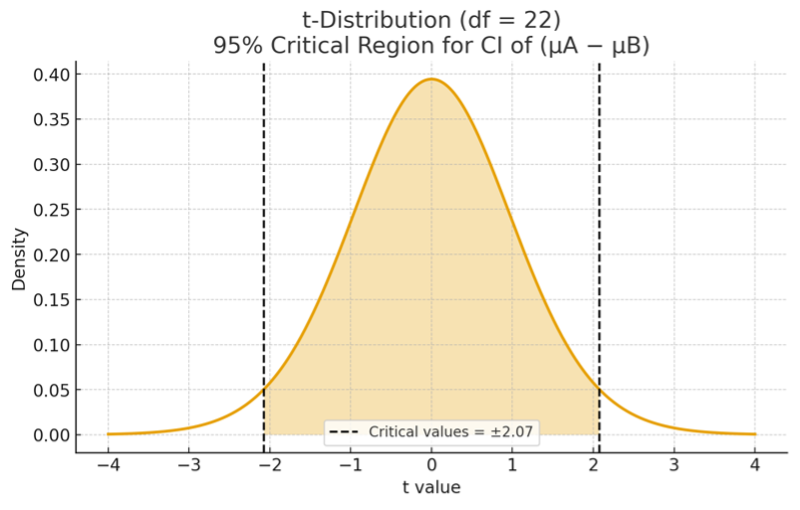
\includegraphics[width=1\textwidth,height=\textheight]{Fig/q2_a.png}
\end{frame}

\begin{frame}{Exercise 2 (Cont'd)}
\protect\hypertarget{exercise-2-contd-4}{}
\begin{enumerate}
\setcounter{enumi}{1}
\item
  Using a 5\% level of significance, test whether the two airports
  differ in their true average yearly passenger numbers.

  \pause

  The two samples are independent. The population is normally
  distributed, and the population variances of the two funds are equal.
  Therefore, we can use the \textbf{pooled t-test} for hypothesis
  testing.

  \pause

  We first write down the hypothesis, since we want to test if there is
  a different in true average yearly passenger numbers between the two
  airports, we have:

  \pause

  \[
   \begin{aligned}
   H_0: \mu_A - \mu_B &= 0\\
   H_1: \mu_A - \mu_B &\neq 0
   \end{aligned}
   \]
\end{enumerate}
\end{frame}

\begin{frame}{Exercise 2 (Cont'd)}
\protect\hypertarget{exercise-2-contd-5}{}
\pause

Since the 95\% confidence interval in (a) does not contain zero, we can
reject the \(H_0: \mu_A - \mu_B = 0\) at a 5\% level of significance.
That is, we find evidence that the two airports differ in their true
average yearly passenger numbers.
\end{frame}

\begin{frame}{Exercise 2 (Cont'd)}
\protect\hypertarget{exercise-2-contd-6}{}
\vspace{25pt}


\includegraphics[width=1\textwidth,height=\textheight]{Fig/q2_b.png}
\end{frame}

\begin{frame}{Exercise 3}
\protect\hypertarget{exercise-3}{}
The cost of equity represents the required rate of return that firms
must offer to raise equity capital, where a lower cost implies more
favourable financing conditions. An analyst wants to assess whether
firms have experienced an improvement in their cost of equity after
2020. To investigate this, the analyst collects cost-of-equity data for
15 firms before and after 2020, as shown in Table 1.
\end{frame}

\begin{frame}{Exercise 3 (Cont'd)}
\protect\hypertarget{exercise-3-contd}{}
\bigskip

\begin{longtable}[]{@{}ccc@{}}
\toprule()
Firm & Cost of Equity (Pre 2020) & Cost of Equity (Post 2020) \\
\midrule()
\endhead
1 & 3 & 1 \\
2 & 5 & 6 \\
3 & 4 & 3 \\
4 & 1 & 2 \\
5 & 4 & 7 \\
6 & 8 & 3 \\
7 & 10 & 5 \\
8 & 15 & 8 \\
9 & 2 & 4 \\
10 & 9 & 7 \\
11 & 6 & 4 \\
12 & 3 & 2 \\
13 & 8 & 5 \\
14 & 11 & 7 \\
15 & 10 & 5 \\
\bottomrule()
\end{longtable}
\end{frame}

\begin{frame}{Exercise 3 (Cont'd)}
\protect\hypertarget{exercise-3-contd-1}{}
\begin{enumerate}
\item
  Test whether the cost of equity has improved for these firms after
  2020 using a 1\% level of significance.

  \pause

  We therefore have \(\bar{d} = -2\) and \(s_d^2 = 2.9032^2\). We first
  write down the hypothesis, where we have: \vspace{-5pt}

  \pause

  \[
   \begin{aligned}
   H_0: \mu_d &= 0 \quad \text{(The cost of equity did not improve)} \\
   H_1: \mu_d &< 0 \quad \text{(The cost of equity improved)} 
   \end{aligned}
   \]

  \pause

  Since the data is paired, we can use the \textbf{paired t-test} for
  hypothesis testing. We calculate the \(t\)-test statistic using
  \(\bar{d} = -2\), \(n = 15\), and \(s_d^2 = 2.9032^2\):

  \pause

  \[
   t = \frac{\bar{d} - \mu_d}{s_d / \sqrt{n}}
        = \frac{-2}{\,2.9032 / \sqrt{15}\,}
        \approx -2.668
   \]
\end{enumerate}
\end{frame}

\begin{frame}{Exercise 3 (Cont'd)}
\protect\hypertarget{exercise-3-contd-2}{}
\pause

The significance level is \(\alpha=1\%\). To find the critical value for
rejecting the null at this significance level, we look for the
probability of 0.01 in the Student's t-distribution table with a degree
of freedom \(df=n-1=15-1=14\). For a left-tailed test, we look for the
value \(t\) such that the probability to its left is 0.01. From the
table, we find that \(Pr(T <-2.624)= 0.01\). Therefore, the critical
value for a left-tailed test at the 1\% significance level is -2.624.
Since the \(t\)-test statistic (-2.668) is \emph{less} than the critical
value (-2.624), we reject the null hypothesis at the 1\% level of
significance. This suggests there is support for the claim that the cost
of equity has improved after 2020.
\end{frame}

\begin{frame}{Exercise 3 (Cont'd)}
\protect\hypertarget{exercise-3-contd-3}{}
\vspace{25pt}

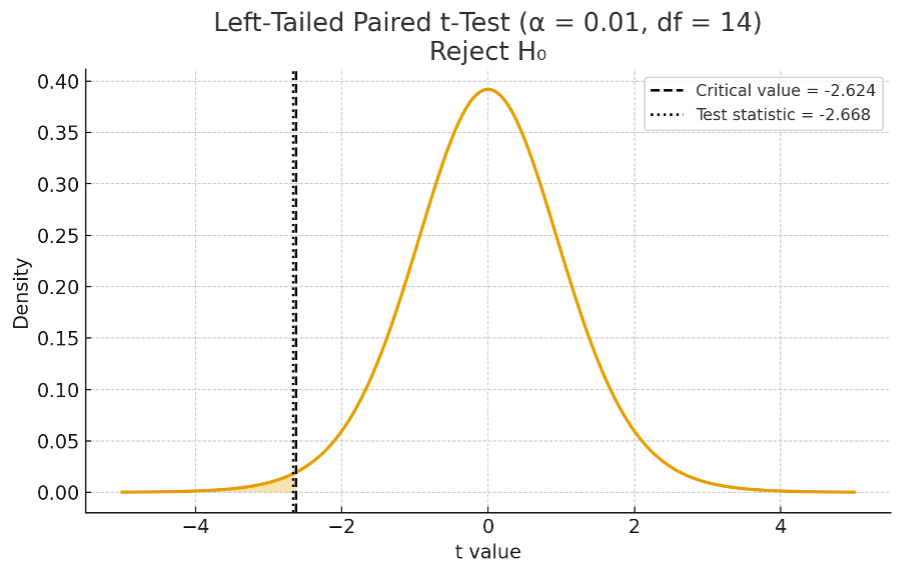
\includegraphics[width=1\textwidth,height=\textheight]{Fig/q3_a.png}
\end{frame}

\begin{frame}{Exercise 3 (Cont'd)}
\protect\hypertarget{exercise-3-contd-4}{}
\begin{enumerate}
\setcounter{enumi}{1}
\item
  Based on your result in part (a), discuss whether any conclusion would
  change if the test were conducted at the 5\% level of significance
  instead. Explain your reasoning.

  \pause

  Since we reject the null at 1\% level of significance in (a), we must
  be able to reject the same null at 5\% level of significance which
  requires a less extreme test statistic to reject the null hypothesis.
\end{enumerate}
\end{frame}

\begin{frame}{Exercise 3 (Cont'd)}
\protect\hypertarget{exercise-3-contd-5}{}
\vspace{25pt}


\includegraphics[width=1\textwidth,height=\textheight]{Fig/q3_b.png}
\end{frame}

\begin{frame}{Exercise 4}
\protect\hypertarget{exercise-4}{}
A university is interested in the well-being of its students and
conducts a survey. Well-being is measured on a scale from 0 to 10. A
sample of 1,000 male students reports an average wellbeing score of 6
with a standard deviation of 2. A separate sample of 1,000 female
students reports an average well-being score of 6.1 with a standard
deviation of 1. Assume the scores are normally distributed and that the
population variances for male and female students are not equal.

\begin{enumerate}
\item
  Test whether the average well-being score of male students is
  different from that of female students at the 5\% level of
  significance.

  \pause

  The two samples are independent. The population is normally
  distributed, and the population variances of the two samples are
  unequal. Therefore, we can use the \textbf{Welch's t-test} for
  hypothesis testing.
\end{enumerate}
\end{frame}

\begin{frame}{Exercise 4 (Cont'd)}
\protect\hypertarget{exercise-4-contd}{}
\pause

We first write down the hypothesis, since we want to test for
differences in wellbeing of male and female students, we have:
\vspace{-2pt}

\pause

\[
\begin{aligned}
H_0: \mu_M - \mu_F &= 0 \\
H_1: \mu_M - \mu_F &\neq 0
\end{aligned}
\]

\pause

Next, we compute the t-test statistic with \(\bar{x}_M = 6\),
\(\bar{x}_F = 6.1\), \(s_M^2 = 2^2\), \(s_F^2 = 1^2\), and
\(n_M = n_F = 1000\):

\pause

\[
\frac{\bar{x}_M - \bar{x}_F}
     {\sqrt{\frac{s_M^2}{n_M} + \frac{s_F^2}{n_F}}}
=
\frac{6 - 6.1}{\sqrt{\frac{2^2}{1000} + \frac{1^2}{1000}}}
\approx -1.41
\]
\end{frame}

\begin{frame}{Exercise 4 (Cont'd)}
\protect\hypertarget{exercise-4-contd-1}{}
\pause

Since the sample size is large, Student's t-distribution converges to
the Standard normal distribution. The significance level is \(\alpha=5%
\). To find the critical value for rejecting the null at this
significance level, we look for the probability of 0.05 in the Standard
normal table. For a two-tailed test, we look for the value \(t\) such
that the probability to both its left and right is 0.025. From the
table, we find that \(Pr(T <1.96)= 0.975\). Therefore, the critical
value for a two-tailed test at the 5\% significance level is ±1.96.
Since the absolute value of the t-test statistic (1.41) is \emph{less}
than the critical value (1.96), we fail to reject the null hypothesis at
the 5\% level of significance.
\end{frame}

\begin{frame}{Exercise 4 (Cont'd)}
\protect\hypertarget{exercise-4-contd-2}{}
\begin{enumerate}
\setcounter{enumi}{1}
\item
  A student union body claims that male and female students are equally
  well in the university. Comment on this claim.

  \pause

  Since we fail to reject the null hypothesis in (a), we can at most say
  we do not find support for a difference in the wellbeing of male and
  female students. We cannot make any claim about the null itself.
\end{enumerate}
\end{frame}

\begin{frame}{Exercise 4 (Cont'd)}
\protect\hypertarget{exercise-4-contd-3}{}
\vspace{25pt}

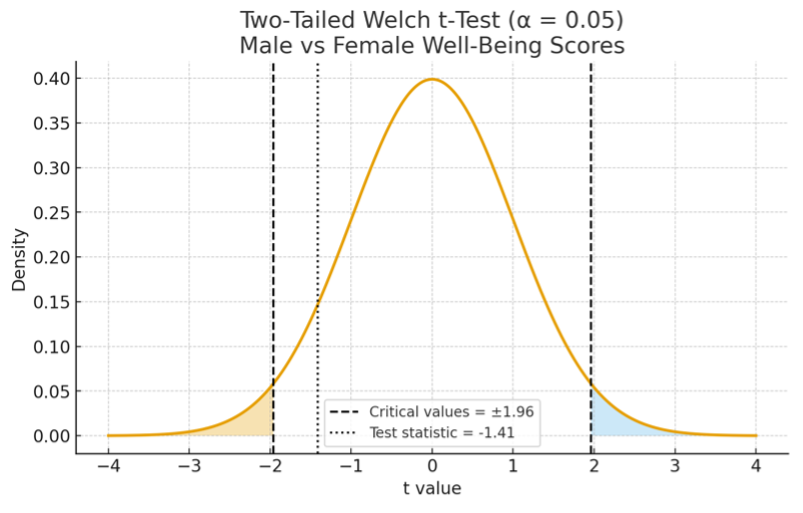
\includegraphics[width=1\textwidth,height=\textheight]{Fig/q4_b.png}
\end{frame}



\end{document}
